\section{Results}\label{results}

\subsection{Lightweight Repeated
Metrics}\label{lightweight-repeated-metrics}

The lightweight repeated experiment provides an initial
development-oriented comparison of the three simulation conditions.
Table~\ref{tab:lightweight-metrics} reports mean and standard deviation
over ten runs.

\begin{longtable}[]{@{}
  >{\raggedright\arraybackslash}p{(\columnwidth - 8\tabcolsep) * \real{0.1579}}
  >{\raggedleft\arraybackslash}p{(\columnwidth - 8\tabcolsep) * \real{0.2105}}
  >{\raggedleft\arraybackslash}p{(\columnwidth - 8\tabcolsep) * \real{0.2105}}
  >{\raggedleft\arraybackslash}p{(\columnwidth - 8\tabcolsep) * \real{0.2105}}
  >{\raggedleft\arraybackslash}p{(\columnwidth - 8\tabcolsep) * \real{0.2105}}@{}}
\caption{Lightweight repeated metrics on AcademicCredentials. Lower is better.}
\label{tab:lightweight-metrics}\\
\toprule\noalign{}
\begin{minipage}[b]{\linewidth}\raggedright
Mode
\end{minipage} & \begin{minipage}[b]{\linewidth}\raggedleft
Trace variant distance
\end{minipage} & \begin{minipage}[b]{\linewidth}\raggedleft
Activity distance
\end{minipage} & \begin{minipage}[b]{\linewidth}\raggedleft
Resource distance
\end{minipage} & \begin{minipage}[b]{\linewidth}\raggedleft
Mean cycle-time relative error
\end{minipage} \\
\midrule\noalign{}
\endhead
\bottomrule\noalign{}
\endlastfoot
\texttt{central\_baseline} & 0.3357 +/- 0.0227 & 0.0988 +/- 0.0105 &
0.7391 +/- 0.0031 & 0.0507 +/- 0.0371 \\
\texttt{agent\_profile} & 0.3281 +/- 0.0242 & 0.0912 +/- 0.0145 & 0.6123
+/- 0.0046 & 0.0413 +/- 0.0249 \\
\texttt{llm\_agent\_proxy} & 0.3271 +/- 0.0100 & 0.0945 +/- 0.0107 &
0.6404 +/- 0.0121 & 0.0362 +/- 0.0247 \\
\end{longtable}

The lightweight results show a trade-off between control-flow, timing,
and resource-distribution behaviour. The LLM-agent proxy has the lowest
mean trace variant distance and mean cycle-time relative error in this
metric set. The agent-profile condition remains best on activity and
resource distribution distance. Thus, a constrained LLM-style local
decision module can be inserted without disrupting basic control-flow or
cycle-time behaviour, but direct statistical resource profiles remain
strong baselines for resource allocation.

\subsection{Formal Chapela-Campa Distance
Metrics}\label{formal-chapela-campa-distance-metrics}

The formal repeated evaluation gives a stricter comparison.
Table~\ref{tab:formal-metrics} reports selected Chapela-Campa distance
measures over ten generated logs per condition.

Figure~\ref{fig:formal-tradeoffs} visualizes the formal metric table on
a common relative scale. Each bar reports the mean distance divided by
the best mean for that metric; the best condition for a metric has value
1.0, and larger values indicate greater distance from the held-out log.

\begin{figure}[htbp]
\centering
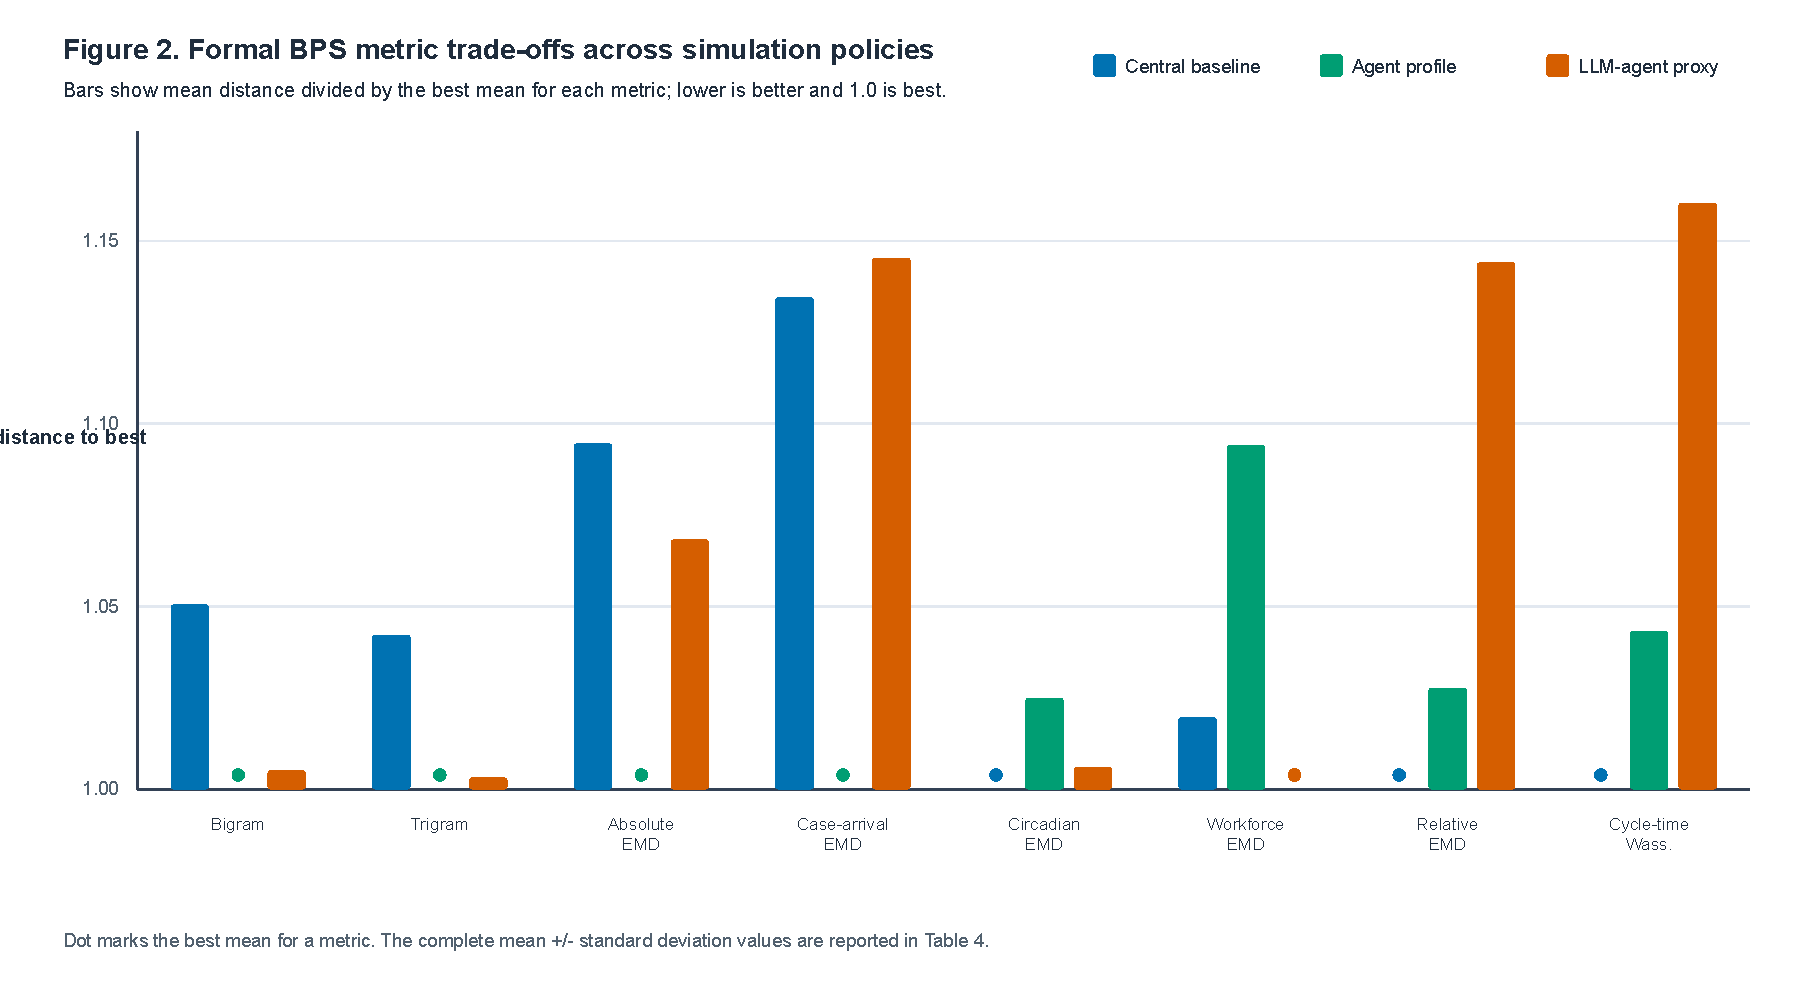
\includegraphics[width=\textwidth]{figures/figure2_formal_metric_tradeoffs.pdf}
\caption{Formal BPS metric trade-offs across simulation policies. Bars show the mean distance divided by the best mean for each Chapela-Campa metric over ten generated logs per condition; lower is better, and stars mark the best mean for each metric. The agent-profile policy is strongest on control-flow n-grams and absolute/case-arrival timing, the LLM-agent proxy is strongest on workforce EMD, and the central baseline is strongest on circadian, relative-event, and cycle-time measures. The figure shows the central empirical pattern: the LLM-agent proxy changes the quality profile, but it does not dominate the statistical baselines.}
\label{fig:formal-tradeoffs}
\end{figure}

\begin{longtable}[]{@{}
  >{\raggedright\arraybackslash}p{(\columnwidth - 8\tabcolsep) * \real{0.1667}}
  >{\raggedleft\arraybackslash}p{(\columnwidth - 8\tabcolsep) * \real{0.2222}}
  >{\raggedleft\arraybackslash}p{(\columnwidth - 8\tabcolsep) * \real{0.2222}}
  >{\raggedleft\arraybackslash}p{(\columnwidth - 8\tabcolsep) * \real{0.2222}}
  >{\raggedright\arraybackslash}p{(\columnwidth - 8\tabcolsep) * \real{0.1667}}@{}}
\caption{Formal BPS quality distances on AcademicCredentials. Lower is better.}
\label{tab:formal-metrics}\\
\toprule\noalign{}
\begin{minipage}[b]{\linewidth}\raggedright
Metric
\end{minipage} & \begin{minipage}[b]{\linewidth}\raggedleft
Central baseline
\end{minipage} & \begin{minipage}[b]{\linewidth}\raggedleft
Agent profile
\end{minipage} & \begin{minipage}[b]{\linewidth}\raggedleft
LLM-agent proxy
\end{minipage} & \begin{minipage}[b]{\linewidth}\raggedright
Best mean
\end{minipage} \\
\midrule\noalign{}
\endhead
\bottomrule\noalign{}
\endlastfoot
Bigram & 0.1618 +/- 0.0093 & 0.1541 +/- 0.0117 & 0.1548 +/- 0.0071 &
\texttt{agent\_profile} \\
Trigram & 0.2065 +/- 0.0126 & 0.1982 +/- 0.0123 & 0.1988 +/- 0.0090 &
\texttt{agent\_profile} \\
Absolute EMD & 159.6972 +/- 95.8036 & 145.9101 +/- 56.3384 & 155.8600
+/- 84.0634 & \texttt{agent\_profile} \\
Case-arrival EMD & 184.3430 +/- 99.4617 & 162.4802 +/- 53.4160 &
186.0864 +/- 90.8550 & \texttt{agent\_profile} \\
Circadian EMD & 3.0208 +/- 0.1159 & 3.0959 +/- 0.3805 & 3.0387 +/-
0.2384 & \texttt{central\_baseline} \\
Workforce EMD & 3.1951 +/- 0.2822 & 3.4284 +/- 0.3764 & 3.1338 +/-
0.3358 & \texttt{llm\_agent\_proxy} \\
Relative EMD & 16.8700 +/- 3.0403 & 17.3357 +/- 4.1486 & 19.3002 +/-
5.1290 & \texttt{central\_baseline} \\
Cycle-time Wasserstein & 16.5231 +/- 2.5704 & 17.2359 +/- 3.4244 &
19.1726 +/- 5.4068 & \texttt{central\_baseline} \\
\end{longtable}

The formal metrics qualify the lightweight result. The agent-profile
condition is best on bigram and trigram distance, indicating slightly
better reproduction of local control-flow patterns. It is also best on
absolute event timing and case-arrival distance. The LLM-agent proxy is
close to the agent-profile baseline on n-gram metrics, but does not
improve absolute timing or case arrivals. Its clearest advantage is
workforce EMD, where it achieves the best mean distance. The central
baseline performs best on circadian event distance, relative event-time
distance, and cycle-time Wasserstein distance.

These results support a dimension-specific claim. The LLM-agent proxy
changes the quality profile of the simulator: it preserves competitive
control-flow behaviour, improves workforce-distance performance in this
experiment, and provides reasoning and handover traces. It does not
improve all temporal distribution measures. A stronger temporal model is
therefore required before an LLM-agent simulator can be claimed to
improve BPS accuracy overall.

\subsection{Robustness Check on AgentSimulator
LoanApp}\label{robustness-check-on-agentsimulator-loanapp}

The second dataset tests whether the result changes for a log with a
clearer resource-role structure than AcademicCredentials. Under the
lightweight metrics, LoanApp is easier to reproduce overall: resource
distribution distances are around 0.04--0.05 rather than above 0.60.
The central baseline has the lowest trace, activity, and resource
distribution distance. The LLM-agent proxy improves on the central
baseline in mean cycle-time relative error and on the agent-profile
policy in resource distribution distance, but it is not best overall.

\begin{longtable}[]{@{}
  >{\raggedright\arraybackslash}p{(\columnwidth - 8\tabcolsep) * \real{0.1800}}
  >{\raggedleft\arraybackslash}p{(\columnwidth - 8\tabcolsep) * \real{0.2050}}
  >{\raggedleft\arraybackslash}p{(\columnwidth - 8\tabcolsep) * \real{0.2050}}
  >{\raggedleft\arraybackslash}p{(\columnwidth - 8\tabcolsep) * \real{0.2050}}
  >{\raggedleft\arraybackslash}p{(\columnwidth - 8\tabcolsep) * \real{0.2050}}@{}}
\caption{AgentSimulator LoanApp robustness results. Lower is better.}
\label{tab:loanapp-robustness}\\
\toprule\noalign{}
\begin{minipage}[b]{\linewidth}\raggedright
Mode
\end{minipage} & \begin{minipage}[b]{\linewidth}\raggedleft
Bigram
\end{minipage} & \begin{minipage}[b]{\linewidth}\raggedleft
Trigram
\end{minipage} & \begin{minipage}[b]{\linewidth}\raggedleft
Workforce EMD
\end{minipage} & \begin{minipage}[b]{\linewidth}\raggedleft
Cycle-time Wasserstein
\end{minipage} \\
\midrule\noalign{}
\endhead
\bottomrule\noalign{}
\endlastfoot
\texttt{central\_baseline} & 0.0288 & 0.0453 & 8.7934 & 67.9520 \\
\texttt{agent\_profile} & 0.0353 & 0.0517 & 8.6541 & 55.4577 \\
\texttt{llm\_agent\_proxy} & 0.0399 & 0.0550 & 8.6489 & 55.6193 \\
\end{longtable}

The formal LoanApp metrics in Table~\ref{tab:loanapp-robustness}
support the same bounded interpretation as the primary dataset. The
central baseline remains best on control-flow n-grams, whereas the
LLM-agent proxy is best on workforce EMD and nearly tied with the
agent-profile policy on cycle-time Wasserstein distance. A separate
LoanApp high-load what-if scenario is more favourable to the LLM-agent
proxy: it has the lowest mean cycle time, lowest p90 cycle time, and
highest throughput. Under the combined reduced-capacity and high-load
stress test, however, the proxy performs worse temporally.
AgentSimulator LoanApp therefore broadens the empirical basis of the
study and reinforces the interpretation of LLM-agent BPS as a
scenario-dependent trade-off.

\subsection{What-If Stress Test}\label{what-if-stress-test}

The previous results evaluate log reproduction. To examine what-if
analysis, an additional stress test adds a simple resource-availability
queue: if a selected resource is still busy or unavailable, the event
waits until that resource becomes available. The intervention constrains
the top 20 high-frequency resources to 50\% capacity and increases
workload by compressing case arrivals with a 1.6x load multiplier. This
combined scenario is not a held-out-log reproduction task; it evaluates
how each policy reacts to a capacity and workload shock.

\begin{longtable}[]{@{}
  >{\raggedright\arraybackslash}p{(\columnwidth - 10\tabcolsep) * \real{0.2100}}
  >{\raggedleft\arraybackslash}p{(\columnwidth - 10\tabcolsep) * \real{0.1580}}
  >{\raggedleft\arraybackslash}p{(\columnwidth - 10\tabcolsep) * \real{0.1580}}
  >{\raggedleft\arraybackslash}p{(\columnwidth - 10\tabcolsep) * \real{0.1580}}
  >{\raggedleft\arraybackslash}p{(\columnwidth - 10\tabcolsep) * \real{0.1580}}
  >{\raggedleft\arraybackslash}p{(\columnwidth - 10\tabcolsep) * \real{0.1580}}@{}}
\caption{What-if stress-test response under reduced capacity and high load on AcademicCredentials. Cycle times are reported in days because the original log contains long waiting intervals.}
\label{tab:what-if}\\
\toprule\noalign{}
\begin{minipage}[b]{\linewidth}\raggedright
Mode
\end{minipage} & \begin{minipage}[b]{\linewidth}\raggedleft
Mean cycle time
\end{minipage} & \begin{minipage}[b]{\linewidth}\raggedleft
P90 cycle time
\end{minipage} & \begin{minipage}[b]{\linewidth}\raggedleft
Handovers per case
\end{minipage} & \begin{minipage}[b]{\linewidth}\raggedleft
Constrained-group share
\end{minipage} & \begin{minipage}[b]{\linewidth}\raggedleft
Throughput
\end{minipage} \\
\midrule\noalign{}
\endhead
\bottomrule\noalign{}
\endlastfoot
\texttt{central\_baseline} & 87.6 & 191.7 & 3.86 & 0.202 & 1.21 \\
\texttt{agent\_profile} & 215.1 & 451.4 & 3.77 & 0.447 & 0.60 \\
\texttt{llm\_agent\_proxy} & 106.4 & 251.8 & 2.09 & 0.366 & 0.93 \\
\end{longtable}

Table~\ref{tab:what-if} differs from the reproduction metrics. The
central baseline has the strongest temporal response in this stress
test, producing the lowest mean and p90 cycle time and the highest
throughput. The LLM-agent proxy does not dominate these temporal
measures, but it substantially reduces handovers per case. The
agent-profile policy relies most heavily on the constrained
high-frequency resource group and shows the largest cycle-time increase.
The stress test therefore captures intervention effects that would be
missed by log similarity alone, including changes in coordination style,
resource concentration, and bottleneck behaviour.

\subsection{Reasoning and Handover
Outputs}\label{reasoning-and-handover-outputs}

The LLM-agent proxy condition produces two artifacts in addition to the
simulated event log. The reasoning log records the local decision
context and selected action for each generated event. The handover log
records transitions between resources when a case moves from one
resource to another. These logs do not directly improve the formal BPS
distance scores, but they increase simulator observability. A generated
event log records what happened; the reasoning and handover logs record
why a local assignment was made and how work moved between resource
agents.
